\documentclass[10pt,spanish,a4paper,openany,notitlepage]{article}
%-------------------------------------Paquetes-----------------------------------------------------------------------
\usepackage[spanish]{babel}  % Traduce los textos a castellano
\usepackage[utf8]{inputenc}	% Permite escribir directamente áéíóúñ
\usepackage{t1enc}            	% Agrega caracteres extendidos al font
\usepackage{amsmath} 		%Permite imprimir mas opcciones matematicas
\usepackage{graphicx}		%Permite agregar imagenes al informe
\usepackage{multicol}  		%Permite dividir el texto en varias columnas
\usepackage{anysize}		%Permite modificar los margenes del documento
\usepackage{float} 			%Permite utilizar H para colocar las imagenes en un lugar especifico 
\usepackage{multirow}		%Permite dividir las tablas en subtablas
\usepackage{booktabs}		%Permiten manejar mejor el tamaño de las tablas
\usepackage{tabulary}		%Permiten manejar mejor el tamaño de las tablas
\usepackage{fancyhdr}		%Permite agregar encabezado y pie fancy
\usepackage{framed}

\usepackage{courier}		%
\usepackage{color}			%
\usepackage{listings}  		%Permite agregar codigo directamente sobre el documento

%---------------------------------------Definiciones propias---------------------------------------------------------
\newcommand{\grad}{\hspace{-2mm}$\phantom{a}^{\circ}$} %El º que no existe como comando
\newcommand{\oiint}{\displaystyle\bigcirc\!\!\!\!\!\!\!\!\int\!\!\!\!\!\int} %Integral doble cerrada
%------------------------------------------------------------------------------------------------------------------------

%-------------------------------------Configuracion De Codigo----------------------------------
\definecolor{dkgreen}{rgb}{0,0.6,0}
\definecolor{gray}{rgb}{0.5,0.5,0.5}

\lstset{language=C,
	breaklines=true,
	keywordstyle=\bf\color{blue},
	commentstyle=\tt\it\color{dkgreen},
	stringstyle=\color{gray},
 	numbers=left,
	numberstyle=\tiny\color{black},
	stepnumber=2,
	numbersep=8pt,
	backgroundcolor=\color{white},
	tabsize=4,
	showspaces=false,
	inputencoding=latin2,
	showstringspaces=false}

\newcommand{\captionlisting}[2][]{%
    \lstinputlisting[caption={\large{\detokenize{#2}}},#1]{#2}%
}

\renewcommand\lstlistingname{Archivo}
%%%%%%%%%%%%%%%%%%%%%%%%%%%%%%%%%%%%%%%%%%%%%%%%%%%

% Título principal del documento.
\title{\textbf{TP0}\\ Generador de fractales de Mandelbrot}

% Información sobre los autores.
\author{Gallipi Leandro, \textit{Padrón Nro. 00000}                    \\
            \texttt{ dirección de e-mail }                                              			\\
            Martinez Gaston Alberto, \textit{Padrón Nro. 91383}                     	\\
            \texttt{gaston.martinez.90@gmail.com}                                            			\\
            Nombre y Apellido de Autor, \textit{Padrón Nro. 00000}                     	\\
            \texttt{ dirección de e-mail }                                              			\\[2.5ex]
            \normalsize{Grupo Nro. ? - 2do. Cuatrimestre de 2014}                       	\\
            \normalsize{66.20 Organización de Computadoras - Práctica Martes}  	\\
            \normalsize{Facultad de Ingeniería, Universidad de Buenos Aires}     	\\
       }
\date{}

\begin{document}
\setcounter{page}{0} %De esta manera no se numera la carátula

\maketitle

% Quita el número en la primer página.
\thispagestyle{empty}

% Resumen
\begin{abstract}
El presente trabajo busca, mediante la implementando un programa que genera fractales, familiarizarse con las herramientas de software que usaremos en los siguientes trabajos.\\
Para ello, se desarrollara en C y se vera su portabilidad entre sistemas con una arquitectura i386 / Amd64 y una arquitectura MIPS32
\end{abstract}
 
\newpage

\section{Introducción}

\section{Desarrollo}

\section{Compilacion}

El presente trabajo incluye un script de \textit{Makefile} para realizar la compilacion de manera automatica. Suponiendo que se este en un sistema Linux con la herramienta \textit{make} instalada \footnote{La misma esta presente en la mayoria de los sistemas Linux, pero pude que requiera ser instalada manualmente} para compilar el trabajo solo es necesario ejecutar:

\begin{framed}
\begin{verbatim}    $ make\end{verbatim}
\end{framed}

Ademas, se provee de un comando para la limpieza de los archivos extras y el ejecutable. El mismo se ejecuta mediante el comando:

\begin{framed}
\begin{verbatim}    $ make clean\end{verbatim}
\end{framed}

\section{Ejecuciones de prueba}

\begin{enumerate}

\item Ejecucion normal 
\begin{framed}
\begin{verbatim}$ ./tp \end{verbatim}
\end{framed}

Genera por defecto el archivo \texttt{out.pgm} con el fractal de mandelbrot centrado en el 0+0i, en un espacio de 4x4, con una resolucion de 640x480. (Figura \ref{test1} Pag \pageref{test1})

\begin{figure}[hbt]
\centering
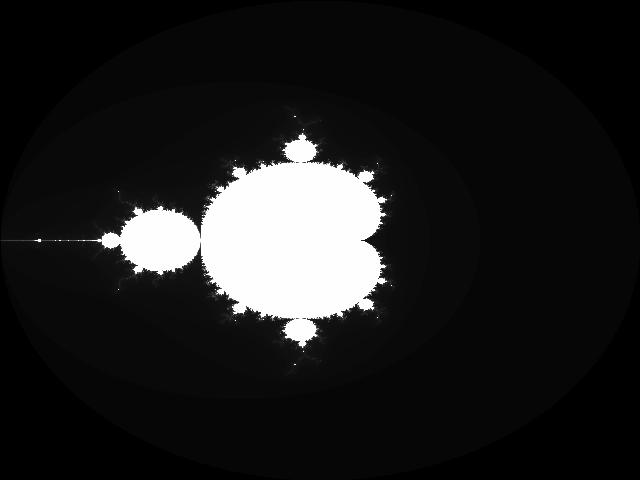
\includegraphics[width=0.25\textwidth]{out.jpg}
\caption{out.pgm}
\label{test1}
\end{figure}

\item Ejecucion reducida
\begin{framed}
\begin{verbatim}$ ./tp -r 30x30 \end{verbatim}
\end{framed}

Genera por defecto el archivo \texttt{out.pgm} con el fractal de mandelbrot centrado en el 0+0i, en un espacio de 4x4, con una resolucion de 30x30. (Figura \ref{test2} Pag \pageref{test2})

\begin{figure}[hbt]
\centering

\includegraphics[]{out2.jpg}
\caption{out.pgm}
\label{test2}
\end{figure}

\item Ejecucion desplazada 1
\begin{framed}
\begin{verbatim}$ ./tp -c 1+0i \end{verbatim}
\end{framed}

Genera por defecto el archivo \texttt{out.pgm} con el fractal de mandelbrot centrado en el 1+0i, en un espacio de 4x4, con una resolucion de 640x480. (Figura \ref{test3} Pag \pageref{test3})

\begin{figure}[hbt]
\centering
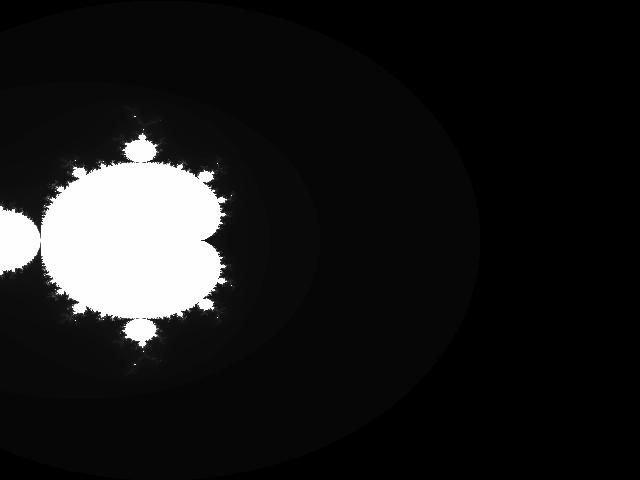
\includegraphics[width=0.25\textwidth]{out3.jpg}
\caption{out.pgm}
\label{test3}
\end{figure}

\item Ejecucion desplazada 2
\begin{framed}
\begin{verbatim}$ ./tp -c 0-1i \end{verbatim}
\end{framed}

Genera por defecto el archivo \texttt{out.pgm} con el fractal de mandelbrot centrado en el 1+0i, en un espacio de 4x4, con una resolucion de 640x480. (Figura \ref{test4} Pag \pageref{test4})

\begin{figure}[hbt]
\centering
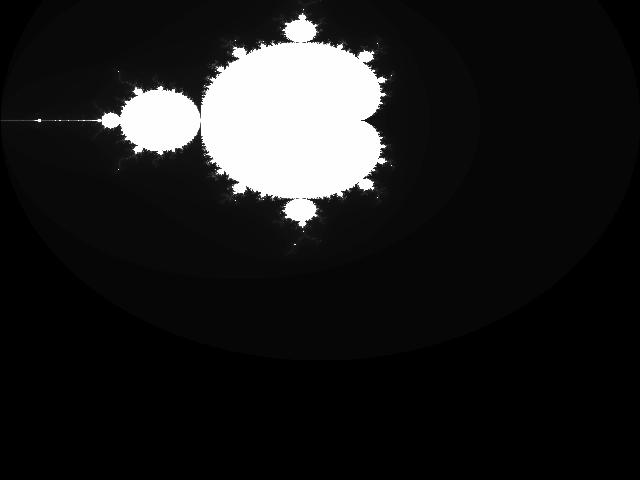
\includegraphics[width=0.25\textwidth]{out4.jpg}
\caption{out.pgm}
\label{test4}
\end{figure}

\item Ejecucion deformada 1
\begin{framed}
\begin{verbatim}$./tp -H 2\end{verbatim}
\end{framed}

Genera por defecto el archivo \texttt{out.pgm} con el fractal de mandelbrot centrado en el 0+0i, en un espacio de 2x4, con una resolucion de 640x480. (Figura \ref{test5} Pag \pageref{test5})

\begin{figure}[hbt]
\centering
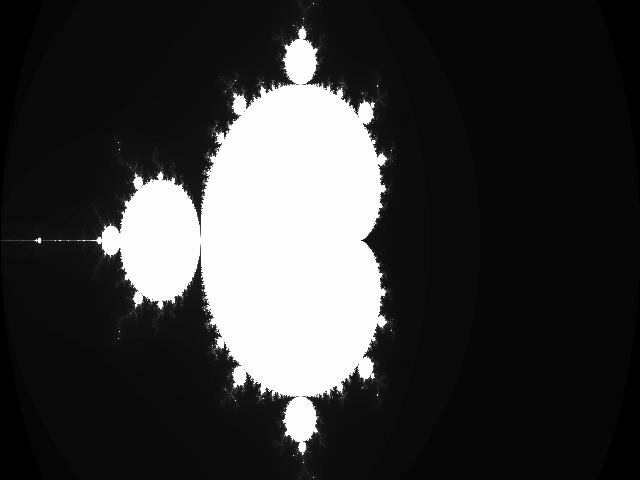
\includegraphics[width=0.25\textwidth]{out5.jpg}
\caption{out.pgm}
\label{test5}
\end{figure}

\item Ejecucion deformada 2
\begin{framed}
\begin{verbatim}$./tp -w 2\end{verbatim}
\end{framed}

Genera por defecto el archivo \texttt{out.pgm} con el fractal de mandelbrot centrado en el 0+0i, en un espacio de 4x2, con una resolucion de 640x480. (Figura \ref{test6} Pag \pageref{test6})

\begin{figure}[hbt]
\centering
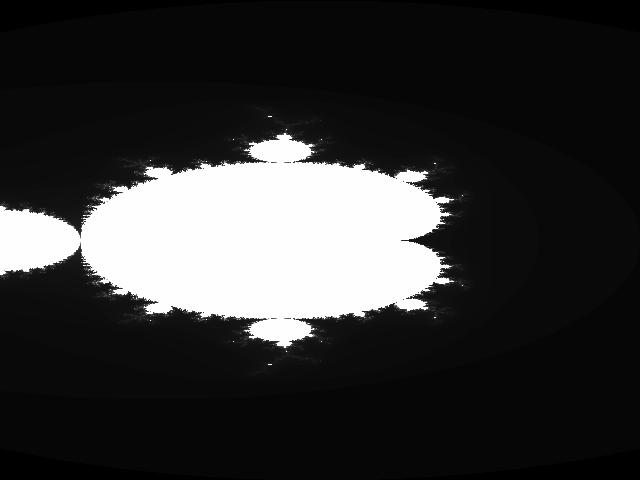
\includegraphics[width=0.25\textwidth]{out6.jpg}
\caption{out.pgm}
\label{test6}
\end{figure}


\item Ejecucion deformada combinada 1
\begin{framed}
\begin{verbatim}$./tp -H 2 -r 240x480\end{verbatim}
\end{framed}

Genera por defecto el archivo \texttt{out.pgm} con el fractal de mandelbrot centrado en el 0+0i, en un espacio de 4x2, con una resolucion de 240x480. (Figura \ref{test7} Pag \pageref{test7})

\begin{figure}[hbt]
\centering
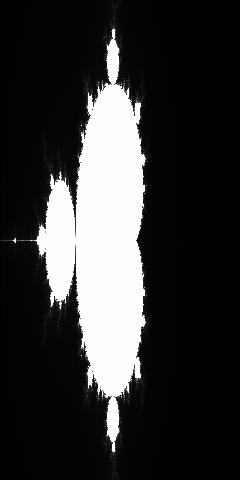
\includegraphics[width=0.25\textwidth]{out7.jpg}
\caption{out.pgm}
\label{test7}
\end{figure}

\item Ejecucion deformada combinada 2
\begin{framed}
\begin{verbatim}$./tp -w 2 -r 600x100\end{verbatim}
\end{framed}

Genera por defecto el archivo \texttt{out.pgm} con el fractal de mandelbrot centrado en el 0+0i, en un espacio de 4x2, con una resolucion de 600x100. (Figura \ref{test8} Pag \pageref{test8})

\begin{figure}[hbt]
\centering

\includegraphics[width=0.25\textwidth]{out8.jpg}
\caption{out.pgm}
\label{test8}
\end{figure}

\item Ejecucion con zona amplificada
\begin{framed}
\begin{verbatim}$./tp -c +0.282-0.01i -w 0.005 -H 0.005 -r 1000x1000\end{verbatim}
\end{framed}

Genera por defecto el archivo \texttt{out.pgm} con el fractal de mandelbrot centrado en el 0.282-0.01i, en un espacio de 0.005x0.005, con una resolucion de 1000x1000. (Figura \ref{test9} Pag \pageref{test9})

\begin{figure}[hbt]
\centering
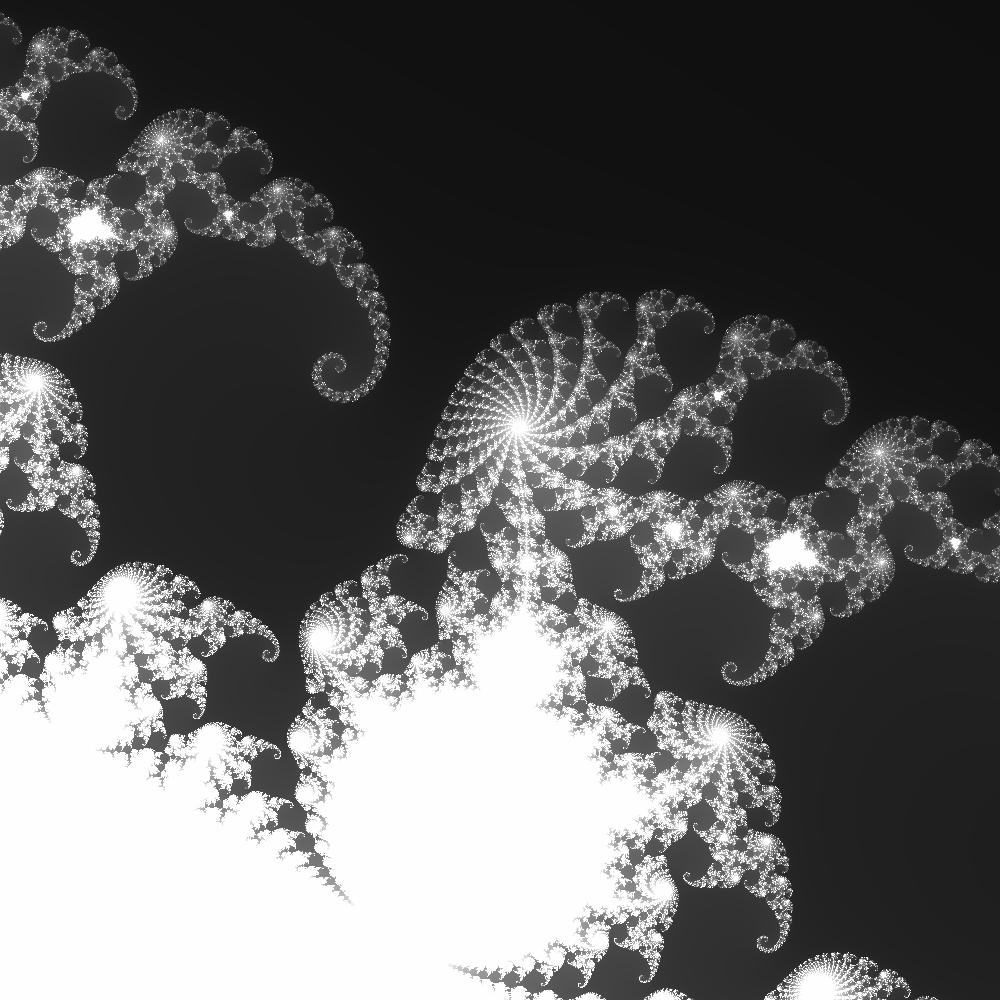
\includegraphics[width=0.25\textwidth]{out9.jpg}
\caption{out.pgm}
\label{test9}
\end{figure}

\item Ejecucion por consola 1
\begin{framed}
\begin{verbatim}$./tp -r 1x1 -o -\end{verbatim}
\end{framed}
Da como resultado la siguiente salida
\begin{framed}
\begin{verbatim}P2
1
1
255
0\end{verbatim}
\end{framed}
Notar que el pixel es 0 (negro) ya que la mayoria de la zona barrida en las dimensiones por defecto son de ese color.


\item Ejecucion por consola 2
\begin{framed}
\begin{verbatim}$./tp -r 1x1 -w 0.0001 -H 0.0001 -o -\end{verbatim}
\end{framed}
Da como resultado la siguiente salida
\begin{framed}
\begin{verbatim}P2
1
1
255
255 \end{verbatim}
\end{framed}
En este caso, el pixel es 255 (blanco) ya que pertenece al centro del conjunto que es completamente blanco.


%\$ ./tp --help
%Usage: tp 	[option_1 opt_arg1 option_2 opt_arg2 ...]
%		[-o|--output] <output_file>
%		[-r|--resolution] <pixel_width>x<pixel_height>
%		[-c|--center] <real_center>[+|-]<imaginary_center>i
%		[-w|--width] <width>
%		[-H|--height] <height>
%		[-h|--help]


\end{enumerate}




\newpage
\appendix
\section{Codigo C}

\captionlisting{tp.c}

\newpage
\section{Makefile}

\lstinputlisting[language=make,
			breaklines=true,
			keywordstyle=\bf\color{blue},
			commentstyle=\tt\it\color{dkgreen},
			stringstyle=\color{gray},
 			numbers=left,
			numberstyle=\tiny\color{black},
			stepnumber=1,
			numbersep=8pt,
			backgroundcolor=\color{white},
			tabsize=4,
			showspaces=false,
			showstringspaces=false]{Makefile}

\newpage
% Citas bibliográficas.
\begin{thebibliography}{99} %Hasta 99 

\bibitem{?}

\end{thebibliography}

\end{document}
